\chapter{The \fshark{} Compiler and Wrapper}
\section*{Introduction}
\label{sec:fsharkcompiler}
Parsing and building a regular F\# program is trivial when using official build tools like
\texttt{msbuild} or \texttt{fsharpc}.
But in the case of \fshark{}, we are not interested in the final result from the
F\# compiler, but merely its half-finished product.

As the F\# Software Foundation offers the official F\# Compiler as a freely
available NuGet package for F\# projects, we can use this package
\texttt{FSharp.Compiler.Services} to parse the entire input \fshark{} program and
give us a Typed Abstract Syntax Tree of the FSharp expressions therein.

The F\# Software Foundation actively encourages developers to create projects
using the F\# compiler library, they have published the collected F\# compiler
as a NuGet package, alongside a tutorial\ref{fsharptutorial}on the usage of the
various compiler parts.

For \fshark{}, the Compiler Services package is used to compile a Typed Abstract
Syntax Tree from a wellformed \fshark{} source code file, which we then
convert into- and print as a valid Futhark program.
The Typed Abstract Syntax Tree is merely an AST that already has tagged all the
contained expressions with their respective types.

We'll start with a detailed explanation of the \fshark{} Compiler Pipeline.

\subsection*{The \fshark{} Compiler Pipeline in practice}
To examine the compiler pipeline in action, we'll go through the motions with
the small example program displayed in figure \ref{fig:fsharkusageexample}.

\begin{figure}[h]
  \centering
    \begin{minted}[linenos,breaklines]{fsharp}
module FSharkExample
open FShark.Main

[<EntryPoint>]
let main argv =
  let wrapper = 
    new FSharkWrapper(
      libName="ExampleModule",
      tmpRoot="/home/mikkel/FShark",
      preludePath= "/home/mikkel/Documents/fshark/FSharkPrelude/bin/Debug/FSharkPrelude.dll",
      openCL=true,
      unsafe=true,
      debug=false
      )
  wrapper.AddSourceFile "../../srcs/ExampleModule.fs"
  wrapper.CompileAndLoad
  let xs = [|1;2;3;4|]
  let input = [|xs|] : obj array
  let xs' = wrapper.InvokeFunction "MapPlusTwo" input :?> int array
  printfn "Mapping (+2) over %A gives us %A" xs xs'
  0
    \end{minted}
  \caption{An F\# program using \fshark{}}
  \label{fig:fsharkusageexample}
\end{figure}

We begin by constructing an instance of the \fshark{}Wrapper. It has the following
mandatory arguments:

\begin{description}
\item[\texttt{libName}]\hfill\\
  This is the library name for the \fshark{} program. In the final Futhark
  \texttt{.cs} and \texttt{.dll} files, the main class will have the same name
  as the \texttt{libName}. This doesn't really matter if \fshark{} is just used
  as a JIT compiler, but it's good to have a proper name if the user only wants
  to use the compiler parts of \fshark{}.

\item[\texttt{tmpRoot}]\hfill\\
  The \fshark{} compiler works in its own temporary directory. This argument must
  point to a directory where F\# can write files and execute subprocesses
  (Futhark- and C\# compilers) which also has to write files.
  
\item[\texttt{preludePath}]\hfill\\
  The \fshark{} compiler needs the FShark prelude available to compile FShark
  programs. 

\item[\texttt{openCL}]\hfill\\
  Although Futhark (and therefore \fshark{}) is most effective on OpenCL-enabled
  computers, the benchmarks in \ref{sec:benchmarks} still show a significant
  speed increase for non-OpenCL Futhark over native F\# code.
  Therefore, \fshark{} is also available for non-OpenCL users. Use this flag to
  tell \fshark{} whether Futhark should compile C\# with or without OpenCL.
  
\item[\texttt{unsafe}]\hfill\\
  For some Futhark programs, the Futhark compiler itself is unable to tell
  whether certain array operations or SOAC usages are safe, and will stop the
  compilation, even though the code should (and does) indeed work.
  To enable these unsafe operations, pass a \texttt{true} flag to the compiler.

\item[\texttt{debug}]\hfill\\
  Passing the debug flag to the \fshark{} compiler enables various runtime
  debugging features, for instance benchmarking the time it takes to run various
  parts of the compiler.
\end{description}

Now, we can pass a source file to the \fshark{} wrapper, compile\footnote{See
  subsection \ref{subsec:fsharkwrappercompiles}} it and load it into the \fshark{} wrapper object.

To use the compiled \fshark{} function, we must first wrap our designated input in
an \texttt{obj array}. In this case, our chosen \fshark{} function takes one
argument, an \texttt{int array}. We define this array, and construct an argument
array containing this single element. If the \fshark{} function takes two
arguments, we define an input \texttt{obj array} with two elements, and so
forth.
It is important to declare the input array as an \texttt{obj array}. Otherwise,
F\#s own type checker might very well faultily infer the input array as
something else. In this particular case, \texttt{input} would've been inferred
as being an \texttt{int array array}, until we declared its type specifically.

We then invoke the desired function through the wrapper. As all
reflection-invoked functions return a value of type \texttt{obj}, we need to
downcast this object manually.
In this example, we use F\#s downcast operator \texttt{(:?>)} to declare the
return value as an \texttt{int array}. The actual return type is always the same as the
return type declared in the source \fshark{} file.

\subsection*{When \fshark{} Wrapper Compiles}
\label{sec:fsharkwrappercompiles}
The general way to compile and load an \fshark{} program into the FShark Wrapper,
is by adding \fshark{} source files to the wrapper object by calling the
\texttt{AddSourceFile} method, and followingly calling the \texttt{CompileAndLoad}
method. Although the \fshark{} wrapper also offers other methods of loading and
compilation, this is the primary one, as it initiates the entire \fshark{}
compilation pipeline.

\begin{figure}[h]
  \centering
  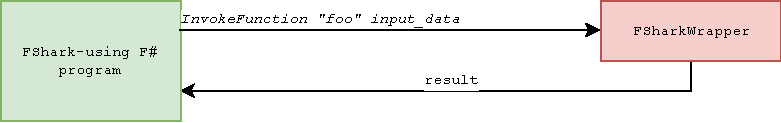
\includegraphics{chapters/figs/csharp/pipeline_step_3.pdf}
  \caption{The \fshark{} compilation pipeline}
  \label{fig:fsharkcompilerpipeline}
\end{figure}


When calling \texttt{CompileAndLoad}, the supplied \fshark{} source files are
concatenated into one long source file, and written to a temporary location.
An FSharpChecker is then initialized, so we can parse and type check the
concatenated source code. The FSharpChecker is a class exported by the FSharp
Compiler Services, and is a class that lets developers use part of the F\#
compilation pipeline at runtime.

We supply the FSharpChecker with the path to our precompiled \fshark{}Prelude
assembly, and then call its \texttt{ParseAndCheckProject} method on to receive
an assembly value, which contains the complete Typed Abstract Syntax Tree of our
\fshark{} program, in the form of an \texttt{FSharpImplementationFileDeclaration}.

If the \fshark{} developer followed the guidelines to write a well-formed FShark
module, the main declaration of the program, the
\texttt{FSharpImplementationFileDeclaration}, should contain a single
\texttt{FSharpEntity}, which in turn contains all the remaining declarations in
the program.

\subsubsection*{The declaration types within F\#'s Typed AST}
The \texttt{FSharpImplementationFileDeclaration} type has three union cases.
\begin{description}
\item[\texttt{InitAction of FSharpExpr}] \hfill\\
  \texttt{InitAction}s are \fsharpexpr{}s that are executed at the
  initialization of the containing entity. These are not supported in \fshark{}.

\item[\texttt{Entity of FSharpEntity * FSharpImplementationFileDeclaration list}]\hfill\\
  An \texttt{Entity} is the declaration of a type or a module. In the case of
  \fshark{}, three different kinds of entities are supported:
  \begin{description}
  \item[FSharpRecords] are standard record types, and can be translated to
    Futhark records with ease.
    This entity has an empty \texttt{FSharpImplementationFileDeclaration list}.
  \item[FSharpAbbreviations] are type abbreviations, and are easily translated
    into Futhark type aliases.
    This entity has an empty \texttt{FSharpImplementationFileDeclaration list}.
  \item[FSharpModules] are named modules which contains subdeclarations.
    In this case, we retrieve the subdeclarations from the \texttt{FSharpImplementationFileDeclaration list}.
    The \fshark{} compiler supports building FShark modules, but current
    limitations demands that modules are flattened when compiled to Futhark.
    This also means that function name prefixes in function calls are stripped
    when compiled to Futhark.
  \end{description}
\item[\texttt{MemberOrFunctionOrValue of \\ FSharpMemberOrFunctionOrValue *
    FSharpMemberOrFunctionOrValue list list * FSharpExpr}]\hfill\\
  F\# doesn't differ between functions and values, which means that a function
  is merely a value with arguments.
  A pattern matched \texttt{MemberOrFunctionOrValue} value has the form
  \texttt{MemberOrFunctionOrValue (v, args, exp)}, where \texttt{v} contains the
  name and the type of the variable.
  If the \texttt{args} list is empty, \texttt{v} is simply a variable. If not,
  \texttt{v} is a function. \texttt{exp} contains the \fsharpexpr{} that
  \texttt{v} is bound to. An \fsharpexpr{} can be anything from a numeric
  constant to a very long function body.
\end{description}

In figure \ref{fig:validfsharkprogram} we see a small but valid \fshark{} program. It
reads like a regular F\# program, but contains the three vital parts that makes
it usable as an \fshark{} program.

\begin{figure}[h]
  \centering
  \begin{minted}[xleftmargin=5pt,linenos]{fsharp}
    module ExampleModule
    open FSharkPrelude

    module SomeValues =
      let Four : int = 4

      let SomePlus (x : int) (y : int) : int = x + y

    [<FSharkEntry>]
    let TimesTwo (x : int) : int =
      SomeValues.SomePlus x x
  
    [<FSharkEntry>]
    let MapPlusTwo (xs : int array) : int array =
      Map ((+)2) xs

    let PlusSeven (x : int) : int =
      SomeValues.SomePlus x 7
  \end{minted}
  \caption{A valid \fshark{} program}
  \label{fig:validfsharkprogram}
\end{figure}

\begin{itemize}
\item The module declaration on the first line declares that the following code
  is inside a module. In this case, we are declaring the module
  \texttt{ExampleModule}, although we could use any valid F\# module name.
  As shown in figure \ref{fig:validfsharkprogramresult}, the top module
  declaration falls away during compilation, so only the top module contents are
  left.

\item This \texttt{open} statement ensures that the F\# Compiler Services has
  access to the \fshark{}Prelude during the compilation. It is possible to write an
  \fshark{} program which doesn't use the FSharkPrelude, but this removes access to
  the SOACs that we use to write our data parallel programs.

\item The \texttt{[<\fshark{}Entry>]} attributed function \texttt{TimesTwo} ensures
  that the resulting Futhark library from the \fshark{} compiler has at least one
  entry point function.
  Without any entry point functions, we won't have any functions in the final
  compiled \fshark{} program.
\end{itemize}

\begin{figure}
  \centering
\begin{lstlisting}[language=Futhark]
    let Four : i32 = 4i32
    let SomePlus (x : i32) (y : i32) : i32 =
      ((x i32.+ y))
    entry TimesTwo (x : i32) : i32 =
      unsafe SomePlus(x) (x)
    entry MapPlusTwo (xs : []i32) : []i32 =
      unsafe map (let x = 2i32 in
                  (\(y : i32) -> ((x i32.+ y)))) (xs)
    let PlusSeven (x : i32) : i32 =
      SomePlus(x) (7i32)
      \end{lstlisting}
  \caption{A valid \fshark{} program, compiled to Futhark}
  \label{fig:validfsharkprogramresult}
\end{figure}

In figure \ref{fig:validfsharkprogramresult} we see the resulting Futhark program.
For now, we will ignore the transformations that have happened, except for two
things: The \texttt{Map} function (called from \fshark{}Prelude) has been rewritten
as the plain Futhark SOAC \texttt{map} in lowercase, and the module SomeValues has been
flattened (see sec \ref{futurework:modules} for future plans.)

This Futhark program is then stored in a temporary location in the user's file
system, and compiled into as a library, using Futhark's C\# compiler, either
with or without OpenCL support. Finally after this compilation, we can invoke
the resulting .dll file from within the \fshark{}-using F\# program.

\subsection*{Building \fshark{} from the Typed AST}
\label{sec:fsharkcompilerrules}
Only the supported FSharpExpr's has been listed here, but the full range of
FSharpExpr's are available on \cite{typedtree}.

\subsection*{FSharp-to-\fshark{}IL rules}
INTRODUCTION HERE

For these translations, we will disregard that all \fsharpexpr{}s are union
cases of the F\# data type \texttt{BasicPatterns}.


\begin{figure}
  \begin{framed}
    
  \centering
\begin{tabular}{@{}l c l}% to \linewidth {l c X}
  $\evals{Entity(\lit{IsFSharpRecord}, [(field_0 : \tau_0), \ldots, (field_n : \tau_n)])}$ & & \\
  $= \lit{FSharkRecord([}(field_0 : \evals{\tau_0}), \ldots, (field_n : \evals{\tau_n})\lit{])}$ & & \\
  ~ \\
\end{tabular}
\begin{tabular}{@{}l c l}% to \linewidth {l c X}
  $\evals{Entity(\lit{IsFSharpTypeAbbreviation}, alias, \tau)}$ & & \\
  $= \lit{FSharkTypeAlias(} alias, \evals{\tau}\lit{)}$ & & \\
  ~ \\
\end{tabular}
\begin{tabular}{@{}l c l}% to \linewidth {l c X}
  $\evals{Entity(\lit{IsFSharpModule}, [decl_0,\ldots,decl_n])}$ & & \\
  $= [\evals{decl_0},\ldots,\evals{decl_n}]$ & & \\
  ~ \\
\end{tabular}
\begin{tabular}{@{}l c l}% to \linewidth {l c X}
  $\evals{MemberOrFunctionOrValue((name, \tau^{*}, IsEntryFunction), [(arg_0 : \tau_0), \ldots, (arg_n : \tau_n)], e)}$ & & \\
  $= FSharkVal(IsEntryFunction, \lit{FSharkFunction}([\evals{\tau_0}, \ldots, \evals{\tau_n}], \evals{\tau^{*}}),name, [arg_0,..,arg_n],\evals{e})$ & & \\
  ~ \\
\end{tabular}
\caption{Rules for translating FSharp declarations to FShark
    declarations}
  \end{framed}

\end{figure}


\begin{figure}
  \centering
\begin{tabular}{@{}l c l}% to \linewidth {l c X}
  $\evals{System.Int8}$ & $=$ & $\lit{FInt8} $ \\ 
  $\evals{System.Int16}$ & $=$ & $\lit{FInt16}$
  \\
  $\evals{System.Int32}$ & $=$ & $\lit{FInt32} $ \\ 
  $\evals{System.Int64}$ & $=$ & $\lit{FInt64} $
  \\
  $\evals{System.UInt8}$ & $=$ & $\lit{FUInt8} $ \\ 
  $\evals{System.UInt16}$ & $=$ & $\lit{FUInt16} $ 
  \\
  $\evals{System.UInt32}$ & $=$ & $\lit{FUInt32} $ \\ 
  $\evals{System.UInt64}$ & $=$ & $\lit{FUInt64} $ 
  \\
  $\evals{System.Single}$ & $=$ & $\lit{FSingle} $ \\ 
  $\evals{System.Double}$ & $=$ & $\lit{FDouble} $ 
  \\
  $\evals{System.Boolean}$ & $=$ & $\lit{Bool} $ \\ 
  $\evals{System.Array~\tau}$ & $=$ & $\lit{\fshark{}Array }\evals{\tau}$
  \\
  $\evals{System.Tuple~(\tau_0 \times \ldots \times \tau_n)}$ & $=$ & $\lit{\fshark{}Tuple}~(\evals{\tau_0}~\times~\ldots~\times~\evals{\tau_n)}$ \\ ~ \\
\end{tabular}

INSERT NOTE ON RULE FOR TUPLE ('a [] * long [])

\caption{Rules for translating .NET types to FSharkIL types}
\end{figure}

\begin{figure}
  \centering
\begin{tabular}{@{}l c l}% to \linewidth {l c X}
  $\evals{\lit{FInt8}}}$ & $=$ & $\lit{i8} $ \\ 
  $\evals{\lit{FInt16}}$ & $=$ & $\lit{i16}$
  \\              
  $\evals{\lit{FInt32}}$ & $=$ & $\lit{i32} $ \\ 
  $\evals{\lit{FInt64}}$ & $=$ & $\lit{i64} $
  \\
  $\evals{\lit{FUInt8}}$ & $=$ & $\lit{u8} $ \\ 
  $\evals{\lit{FUInt16}}$ & $=$ & $\lit{u16} $ 
  \\               
  $\evals{\lit{FUInt32}}$ & $=$ & $\lit{u32} $ \\ 
  $\evals{\lit{FUInt64}}$ & $=$ & $\lit{u64} $ 
  \\
  $\evals{\lit{FSingle}}$ & $=$ & $\lit{f32} $ \\ 
  $\evals{\lit{FDouble}}$ & $=$ & $\lit{f64} $ \\
  $\evals{\lit{Bool}}$ & $=$ & $\lit{bool} $ \\ 
  $\evals{\lit{FSharkArray}~\tau}$ & $=$ & $\lit{[]}\evals{\tau}$
  \\
  $\evals{\lit{\fshark{}Tuple}~({\tau_0}~\times~\ldots~\times~{\tau_n})}$ & $=$ & $(\evals{\tau_0},\ldots,\evals{\tau_n})$ \\ ~ \\
\end{tabular}
\caption{\texttt{\fshark{}IL} types to Futhark types}
\end{figure}

\begin{figure}
  \centering
  \begin{tabular}{@{}l c l}% to \linewidth {l c X}
  $\evals{Const(obj, \tau)}$ & $=$ & $\lit{Const(}obj, \evals{\tau} \lit{)}$ \\
  $\evals{Value(v)}$ & $=$ & $\lit{Var(}v{)}$ \\
  $\evals{AddressOf(v)}$ & $=$ & $\evals{v}$ \\
  $\evals{NewTuple(\_, [e_0,...,e_1])}$ & $=$ & $\lit{Tuple([}\evals{e_0},\ldots, \evals{e_n}\lit{])}$ \\
  $\evals{NewRecord((v_0 : \tau_0 * \ldots * v_n : \tau_n), [e_0,...,e_1])}$ & $=$ & $\lit{Record([}(v_0,\evals{e_0}),\ldots,(v_n,\evals{e_n})\lit{])}$ \\
  $\evals{NewArray(\tau, [e_0,...,e_1])}$ & $=$ & $\lit{List(}\evals{\tau},\lit{[}\evals{e_0},\ldots, \evals{e_n}\lit{]}\lit{)}$ \\
  $\evals{TupleGet(\_, i, e)}$ & $=$ & $\lit{TupleGet(}\evals{e}, i{)}$ \\
  $\evals{FSharpFieldGet(e, \_, field)}$ & $=$ & $\lit{RecordGet(}field, \evals{e}{)}$ \\
    $\evals{Call(\_, \lit{GetArray}, \_, nil, [e_0, e_1])}$ & $=$ & $\lit{ArrayIndex(}\evals{e_0},\evals{e_1}]\lit{)}$ \\
    $\evals{Call(\_, name, \_, nil, [e_0, \ldots, e_n])}$ & $=$ & $\lit{Call(}name, [\evals{e_0},\ldots,\evals{e_n}]\lit{)}$ \\
    $\evals{Call(\_, name, \_, \tau, [e_0, \ldots, e_n])}$ & $=$ & $\lit{TypedCall(}\evals{\tau},name, [\evals{e_0}, \ldots, \evals{e_n}]\lit{)}$ \\
    $\evals{Call(\_, infixOp, \_, \tau, [e_0, e_1])}$ & $=$ & $\lit{InfixOp(}infixOp, \evals{\tau}, \evals{e_0}, \evals{e_1}\lit{)}$ \\
    $\evals{Call(\_, unaryOp, \_, \tau, [e_0])}$ & $=$ & $\lit{UnaryOp(}unaryOp, \evals{\tau}, \evals{e_0}\lit{)}$ \\
  $\evals{Let(v, e_0, e_1)}$ & $=$ & $\lit{LetIn(}v, \evals{e_0}, \evals{e_1}\lit{)}$ \\
  $\evals{IfThenElse(e_0, e_1, e_2)}$ & $=$ & $\lit{If(}\evals{e_0}, \evals{e_1}, \evals{e_2}\lit{)}$ \\
  $\evals{Lambda((v : \tau), e)}$ & $=$ & $\lit{Lambda(}v, \evals{\tau}, \evals{e} \lit{)}$ \\
  $\evals{Application(func, \_, [e_0, \ldots, e_n])}$ & $=$ & $\lit{Application(}\evals{func}, \lit{[}\evals{e_0},\ldots, \evals{e_n}\lit{])}$ \\
  $\evals{TypeLambda(e)}$ & $=$ & $\evals{e}$ \\
  $\evals{DecisionTree(\_, \_)}$ & $=$ & $\lit{Pass}$ \\
  $\evals{DecisionTreeSuccess(\_, \_)}$ & $=$ & $\lit{Pass}$ \\ ~ \\
\end{tabular}
\caption{Translation rules for FSharp expressions to FSharkIL expressions}
\end{figure}

  
\begin{figure}
  \centering
  \begin{tabular}{@{}l c l}% to \linewidth {l c X}
  $\evals{Const(obj, \tau )}$ & $=$ & $obj\evals{\tau}$ \\
  $\evals{Var(v)}$ & $=$ & $v$\\
  $\evals{Tuple([e_0,\ldots, e_n])}$ & $=$ & $(\evals{e_0},\ldots, \evals{e_n})$\\
  $\evals{Record([(v_0, e_0),\ldots,(v_n,e_n)])}$ & $=$ & $\{v_0=\evals{e_0},~\ldots,~v_n=\evals{e_n}\}$ \\
  $\evals{List(}\evals{\tau},\lit{[}\evals{e_0},\ldots, \evals{e_n}\lit{]}\lit{)}$ & $=$ & $[\evals{e_0},~\ldots,~\evals{e_n}]$\\
  $\evals{TupleGet(}\evals{e}, i{)}$ & $=$ & $\evals{e}.i$ \\
  $\evals{RecordGet(field, e)}$ & $=$ & $\evals{e}.field$ \\
  $\evals{ArrayIndex(e_{arr},[e_0, \ldots, e_n])}$ & $=$ & $\evals{e_{arr}}\lit{[}\evals{e_0},\ldots,\evals{e_n}\lit{]}$ \\
    
  $\evals{Call(name, [e_0,\ldots,e_n]\lit{)}}$ & $=$ & $name~(\evals{e_0})~\ldots~(\evals{e_n})$ \\
  $\evals{TypedCall(}\evals{\tau},name, [\evals{e_0}, \ldots, \evals{e_n}]\lit{)}$ & $=$ & $\evals{\tau}.name~(\evals{e_0})~\ldots~(\evals{e_n})$ \\
  $\evals{InfixOp(}infixOp, \evals{\tau}, \evals{e_0}, \evals{e_1}\lit{)}$ & $=$ & $(\evals{e_0})~\evals{\tau}.infixOp~(\evals{e_1})$ \\
  $\evals{UnaryOp(}unaryOp, \evals{\tau}, \evals{e_0}\lit{)}$ & $=$ & $\evals{\tau}.unaryOp~(\evals{e_0})$ \\

  $\evals{LetIn(}v, \evals{e_0}, \evals{e_1}\lit{)}$ & $=$ & $\mathtt{let}~v~=~\evals{e_0}~\mathtt{in}~\evals{e_1}$ \\

  $\evals{If(}\evals{e_0}, \evals{e_1}, \evals{e_2}\lit{)}$ & $=$ & $\mathtt{if}~\evals{e_0}~\mathtt{then}~\evals{e_1}~\mathtt{else}~\evals{e_2}$ \\

  $\evals{Lambda(v, \evals{\tau}, \evals{e} \lit{)}}$ & $=$ & $\mathtt{\backslash}(v : \evals{\tau})~\mathtt{->}~\evals{e}$ \\
  $\evals{Application(\evals{func}, \lit{[}\evals{e_0},\ldots, \evals{e_n}\lit{])}}$ & $=$ & $(\evals{func})~(\evals{e_0})~\ldots~(\evals{e_n})$ \\
  $\evals{Pass}$ & $=$ & $\epsilon$ $$ \\
\end{tabular}
\caption{\texttt{FSharkIL} expressions to Futhark}
\end{figure}


%%% Local Variables:
%%% mode: latex
%%% TeX-master: "../thesis"
%%% End: